\section{引言}\label{introduction}

\subsection{问题背景与陈述}

探究电信学院大学生应该如何内卷是一个很重要的问题。

这里展示一下如何在本项目中插入图片:

\begin{figure}[hb!]
    \centering
    \subfigure[目标检测]{
    \begin{minipage}[t]{0.22\linewidth}
    \centering
    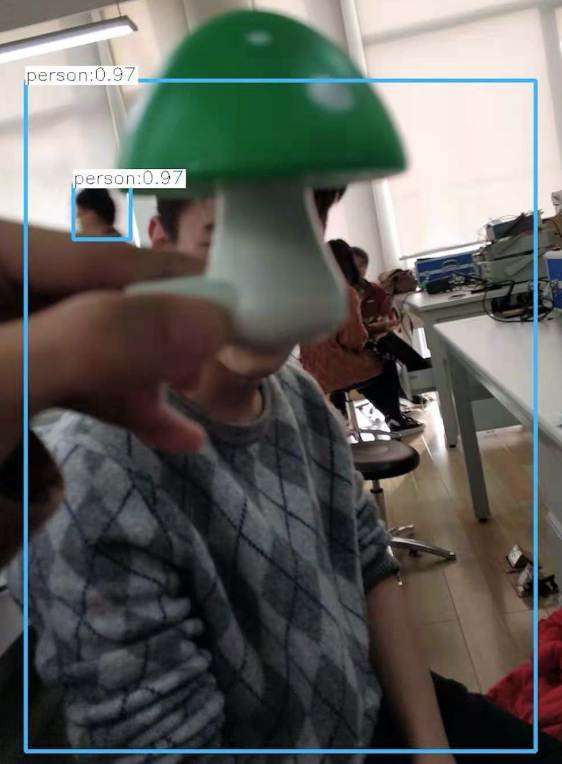
\includegraphics[width=\linewidth]{figures/det.png}
    \end{minipage}\label{fig:det}
    }
    %
    \centering
    \subfigure[语义分割]{
    \begin{minipage}[t]{0.28\linewidth}
    \centering
    
\includegraphics[width=\linewidth]{figures/seg.png}
    \end{minipage}\label{fig:seg}
    }
    %
    \centering
    \subfigure[姿态识别]{
    \begin{minipage}[t]{0.4\linewidth}
    \centering
    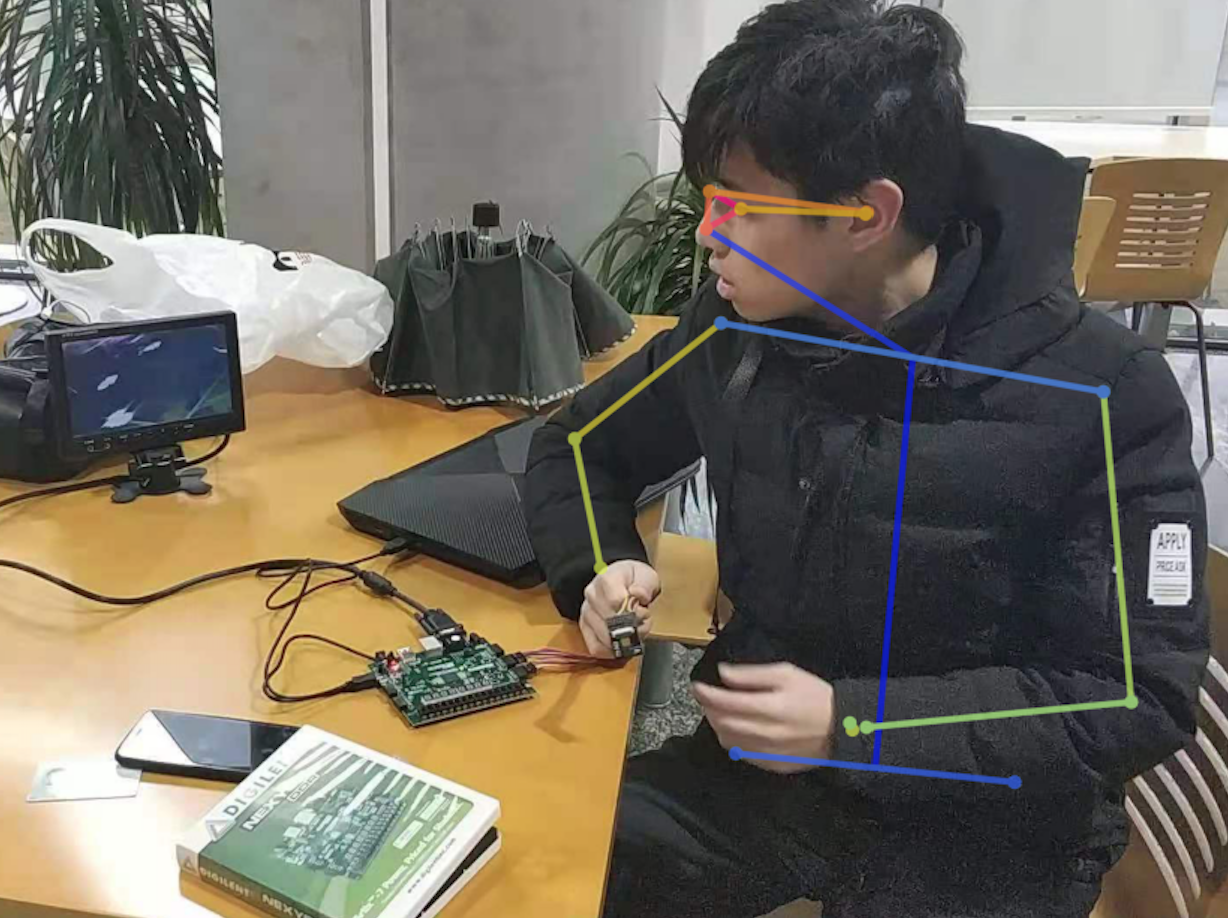
\includegraphics[width=\linewidth]{figures/pose.png}
    \end{minipage}\label{fig:pose}
    }
    %
    \caption{常见视频分析应用图解(图片提供者为中中同学)}\label{fig:cvexample}
    \centering
\end{figure}


\subsection{本文的工作}

本文的工作就是卷字数。

\subsection{文章结构}

采用递进式方法进行卷字数。
